\lecture_date{02/11/2026}

\chapter{Lecture 06}

\section{Review on multivariable calculus (continuation)}

We pickup where we left in \autoref{sec:review-on-multivariable-calculus}. This time our goal is to derive some useful formula to compute directional derivatives, so that we don't have to use \autoref{eq:directional-derivative} each time to evaluate directional derivatives (just like summation, product, chain rule in single variable calculus).

\begin{theorem}[Multivariable chain rule]\label{thm:multivariable-chain-rule}
	Let \( f : \mathbb{R}^n \to \mathbb{R} \) be a function given by
	\[
		f=f(x_1,x_2,\ldots,x_n), \qquad x_i=x_i(t)
	\]

	Then
	\begin{equation}
		\frac{df}{dt} = \sum_{i=1}^{n} \frac{\partial f}{\partial x_i} \frac{dx_i}{dt}.
		\label{eq:multivariable-chain-rule-1}
	\end{equation}
\end{theorem}

This theorem is best understood by practicing some examples.

\begin{example}\label{ex:review-on-multivariable-calculus-continuation-1}
	Let
	\begin{equation}
		f(x,y) = x + y,
		\label{eq:review-on-multivariable-calculus-continuation-1}
	\end{equation}
	where
	\begin{equation}
		\begin{aligned}
			x = e^u & \qquad y = uw,     \\
			u = t^2 & \qquad v = e^t,    \\
			        & \qquad w = \sin t.
		\end{aligned}
		\label{eq:review-on-multivariable-calculus-continuation-2}
	\end{equation}

	We wish to compute $\frac{df}{dt}$ using the multivariable chain rule.

	The following mental picture is useful for efficiently applying the multivariable chain rule: Starting from $f$, follow every possible path to $t$. Along each path, multiply the corresponding partial derivatives, and then add the contributions from all paths.

	\begin{center}
		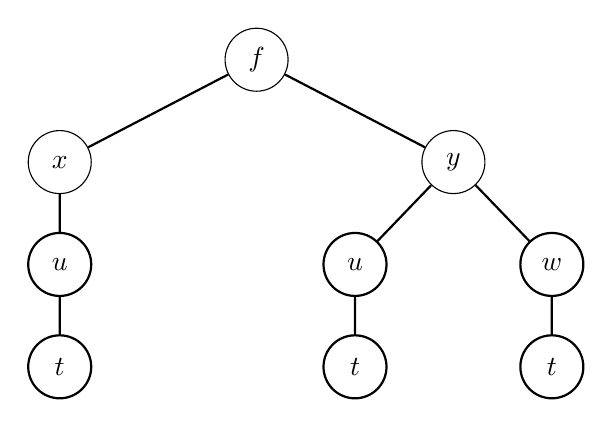
\begin{tikzpicture}[
				level distance=1.3cm,
				every node/.style={
						draw,
						circle,
						minimum size=8mm
					},
				level 1/.style={sibling distance=5cm},
				level 2/.style={sibling distance=2.5cm},
				level 3/.style={sibling distance=1.3cm},
				edge from parent/.style={draw, thick}
			]
			\node {$f$}
			child {
					node {$x$}
					child {
							node {$u$}
							child {node {$t$}}
						}
				}
			child {
					node {$y$}
					child {
							node {$u$}
							child {node {$t$}}
						}
					child {
							node {$w$}
							child {node {$t$}}
						}
				};
		\end{tikzpicture}
	\end{center}

	Therefore, the chain rule gives
	\begin{equation}
		\frac{df}{dt} =
		\frac{\partial f}{\partial x} \frac{d x}{d u} \frac{du}{dt}
		+ \frac{\partial f}{\partial y} \frac{\partial y}{\partial u} \frac{du}{dt}
		+ \frac{\partial f}{\partial y} \frac{\partial y}{\partial w} \frac{dw}{dt}.
		\label{eq:review-on-multivariable-calculus-continuation-3}
	\end{equation}
	Now,
	\[
		\frac{\partial f}{\partial x} =
		\frac{\partial f}{\partial y} = 1,
		\frac{\partial x}{\partial u}=e^u,
		\frac{\partial y}{\partial u}=w,
		\frac{\partial y}{\partial w}=u,
		\frac{du}{dt}=2t,
		\frac{dw}{dt}=\cos t.
	\]

	Substituting everything to \autoref{eq:review-on-multivariable-calculus-continuation-3}, we get

	\begin{equation}
		\frac{df}{dt} = e^u(2t)+w(2t) + u \cos t = 2te^{t^2} + 2t\sin t + t^2 \cos t.
		\label{eq:review-on-multivariable-calculus-continuation-4}
	\end{equation}
\end{example}

To get used to using chain rule from the dependency tree, let's do another example.

\begin{example}\label{ex:review-on-multivariable-calculus-continuation-2}
	Suppose we have a function whose variable dependency tree looks as follows:
	\begin{center}
		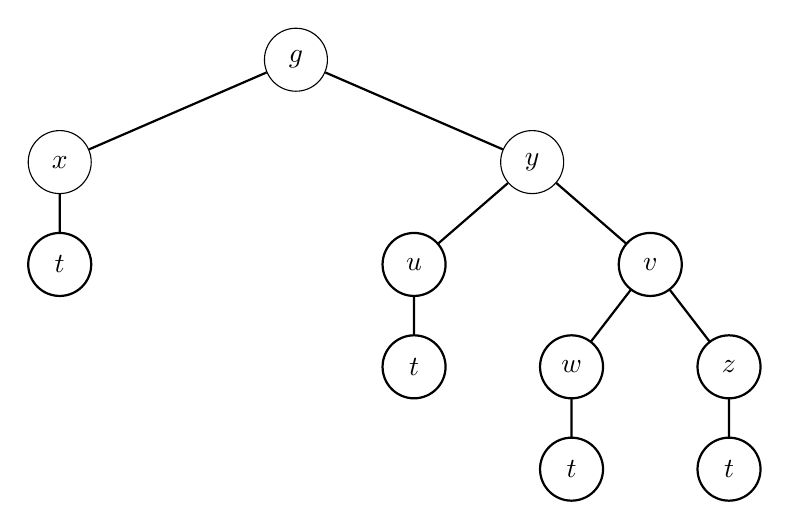
\begin{tikzpicture}[
				level distance=1.3cm,
				every node/.style={
						draw,
						circle,
						minimum size=8mm
					},
				level 1/.style={sibling distance=6cm},
				level 2/.style={sibling distance=3cm},
				level 3/.style={sibling distance=2cm},
				level 4/.style={sibling distance=1cm},
				edge from parent/.style={draw, thick}
			]
			\node {$g$}
			child {
					node {$x$}
					child {node {$t$}}
				}
			child {
					node {$y$}
					child {
							node {$u$}
							child {node {$t$}}
						}
					child {
							node {$v$}
							child {
									node {$w$}
									child {node {$t$}}
								}
							child {
									node {$z$}
									child {node {$t$}}
								}
						}
				};
		\end{tikzpicture}
	\end{center}
	Then
	\begin{equation}
		\frac{dg}{dt} = \frac{\partial g}{\partial x}\frac{dx}{dt}+\frac{\partial g}{\partial y} \frac{\partial y}{\partial u}\frac{du}{dt}+\frac{\partial g}{\partial y} \frac{\partial y}{\partial v} \frac{\partial v}{\partial w}\frac{dw}{dt}+\frac{\partial g}{\partial y} \frac{\partial y}{\partial v} \frac{\partial v}{\partial z}\frac{dz}{dt}.
		\label{eq:review-on-multivariable-calculus-continuation-5}
	\end{equation}
\end{example}

Now we are ready to prove a result that will help us to easily calculate directional derivatives.

\begin{proposition}[Characterisation of directinoal derivatives]\label{prop:review-on-multivariable-calculus-continuation-1}

\end{proposition}
